% Obtención de datos a partir de una muestra del “público objetivo”,
% 	para conocer la relación de éste con el
%	tema tecnológico que se está estudiando.
%
% Observaciones:
%   a) Se puede aplicar diferentes técnicas de obtención de datos:
%	   encuesta, entrevista, focus groups, observación participante, etc.
%
%	   IMPORTANTE: obtener registros audiovisuales (fotos, videos, etc)
%
%   b) El tamaño de la muestra (cantidad de público objetivo), debe ser
%		estimada numéricamente, para que la investigación tenga validez científica.
%
Tomando en cuenta que el presente trabajo conlleva un análisis a el impacto de tecnología
en las colaboraciones internacionales de nuestra universidad, el poder recolectar información
audiovisual como fotos y videos es imposible, debido a que las mayorías de las reuniones son
con personas fuera del país, por lo cual el único material que se presenta es con respecto a
las reuniones acá en la Universidad.

La obtención de datos se realizó a partir del análisis de las reuniones mencionadas anteriormente,
donde se evaluaron los siguientes aspectos:
\begin{itemize}
	% Saber lo que es una teleconferencia, como se usa, cuando hay un error, saber lo que pudo probocarlo
	% Conocer como se realizan las conferencias, como llamar a la gente, como conectarse, etc.
	\item Entendimiento de conceptos tecnológicos.
	% Conocer skype, twiki, lenguajes de programación.
	\item Entendimiento de herramientas tecnológicas.
	% Cuantas veces alguien pide "repetir" lo ultimo que se dijo,
	%  tener la capacidad de explicar conceptos o situaciones técnicas en otros idiomas.
	\item Problemas con el idioma.
	% Que nos dejen hablar y participar en las reuniones
	\item Respeto con todos los colaboradores.
	\item Integración con el equipo de trabajo.
	\item Participación en otros proyectos ya iniciados.
	\item Ayuda sobre proyectos.
	\item Medios de comunicación.
\end{itemize}

Los datos acerca de los puntos anteriores son valores promedios, para los numéricos
y los más frecuentes en caso de ser cualitativos.

\subsection{Encuesta}
La presente encuesta se encuentra disponible en~\footnote{Encuesta Realizada - \url{http://csrg.inf.utfsm.cl/~cmaureir/encuesta.html}},
y los resultados presentados son hasta el \emph{5 de Julio del 2010}~\footnote{Resultados Encuesta - \url{http://csrg.inf.utfsm.cl/~cmaureir/resultados.pdf}}
\begin{enumerate}
    \item ¿Ha trabajo remotamente con otros grupos de trabajo?\\
        R: | Si | No
    \item ¿En promedio, cuantas personas conformaban el grupo trabajo?\\
        R:\\
            | menos de 3\\
            | entre 3 y 5\\
            | entre 6 y 8\\
            | entre 8 y 12\\
            | 12 +
    \item ¿En promedio, cuanto es el tiempo de duración de los
    proyectos o trabajos?\\
        R:\\
            | menos de 1 Mes\\
            | entre 1 y 2 Meses\\
            | entre 3 y 4 Meses\\
            | entre 5 y 10 Meses\\
            | menos de 1 Año\\
            | entre 1 y 2 Años\\
            | más de 2 Años
    % Preguntar por forma de trabajo, jerarquías, etc.
    \item ¿Encuentra que trabajar remotamente beneficia el trabajo en
        equipo?\\
        R: | Si | No
    \item Tecnologías de la Información
    \begin{enumerate}
        \item ¿Cuales de éstas herramientas ha utilizado para trabajar y
            comunicarse remotamente?\\
        R:\\
           | Skype\\
           | Wiki's (Twiki, Mediawiki)\\
           | Aplicaciones web de Manejo de Proyectos (Ej:Trac, Redmine)\\
           | Llamadas telefónicas\\
           | Teleconferencia\\
           | Otra:

        \item ¿Encuentra necesario el uso de tecnologías de la información
        para comunicarse?\\
        R: | Si | No

    \end{enumerate}
    \item Dificultades
    \begin{enumerate}
        \item ¿Ha experimentado problemas de comunicación con el uso de tecnologías?\\
        %\item ¿El idioma ha significado un problema para la comunicación de las partes?
        R: | Si | No
        \item Si es así, seleccione las problemáticas más comunes que ha
        encontrado:\\
        R:\\
	    | Se pide comúnmente que se "repita" lo ultimo que se dijo.\\
	    | Dificultad para explicar o transmitir conceptos o situaciones técnicas.\\
        | Fallas técnicas.\\
        | Otras: 
        \item ¿Lograron solucionar éstos problemas?\\
        R: | Si | No
        \item Si es que pudo, ¿De que manera lo logro?\\
        R:\\
        | Usando otras tecnologías.\\
        | Otra manera:
        \item ¿Considera que el uso de tecnologías mantiene el respeto entre los participantes?\\
        R: | Si | No
        \item ¿Cree que la integridad entre equipos de trabajo se ve afectada negativamente, al sólo tener disponible tecnologías en vez de una comunicación directa?\\
        R: | Si | No
        \item ¿Se ha integrado a equipos de trabajo donde debe en el camino aprender a utilizar tecnologías?\\
        R: | Si | No
        \item Si es así, ¿le ha sido fácil?:\\
        R: | Si | No\\
	\end{enumerate}
    % Cosas que faltan por evaluar:
	%\item Participación en otros proyectos ya iniciados.
\end{enumerate}

\subsection{Resultados}
La presente encuesta fue realizada a personas pertenecientes al estudiantado
de la universidad UTFSM y a miembros del equipo de desarrollo de ALMA-UTFSM
residentes en Chile, EEUU y Alemania.

Total de Personas encuestadas 29 personas.
Se muestran a continuación los resultados de la encuesta, representados en
gráficos de barras para cada pregunta y las respuestas correspondientes a
ella.

\begin{center}
	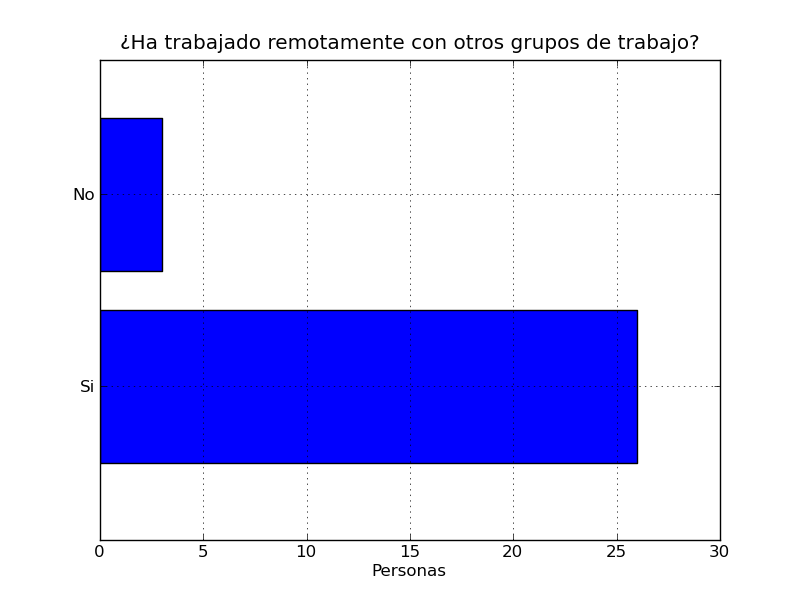
\includegraphics[width=0.8\textwidth]{images/fig1}\\
	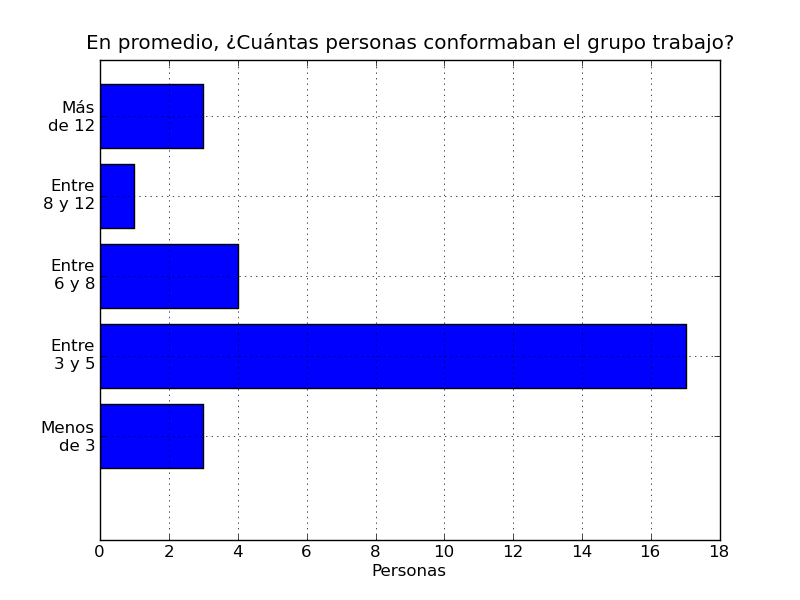
\includegraphics[width=0.8\textwidth]{images/fig2}\\
	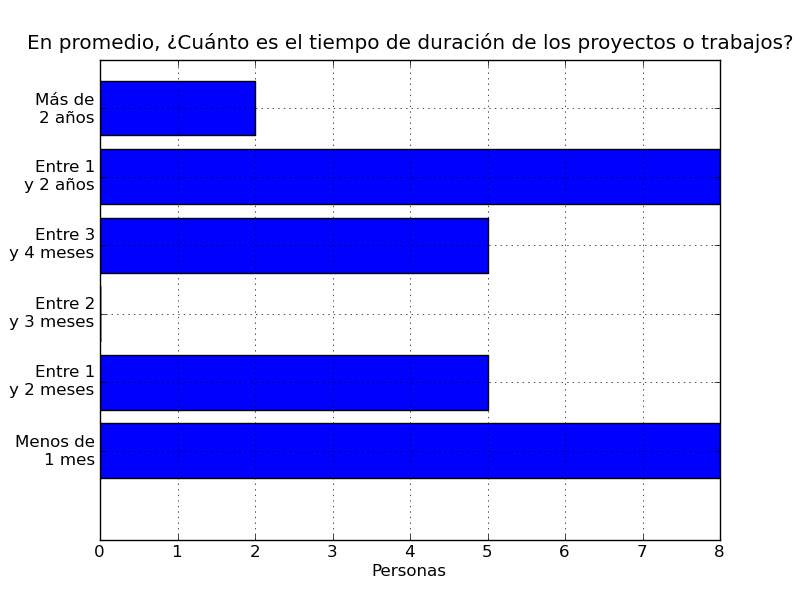
\includegraphics[width=0.8\textwidth]{images/fig3}\\
	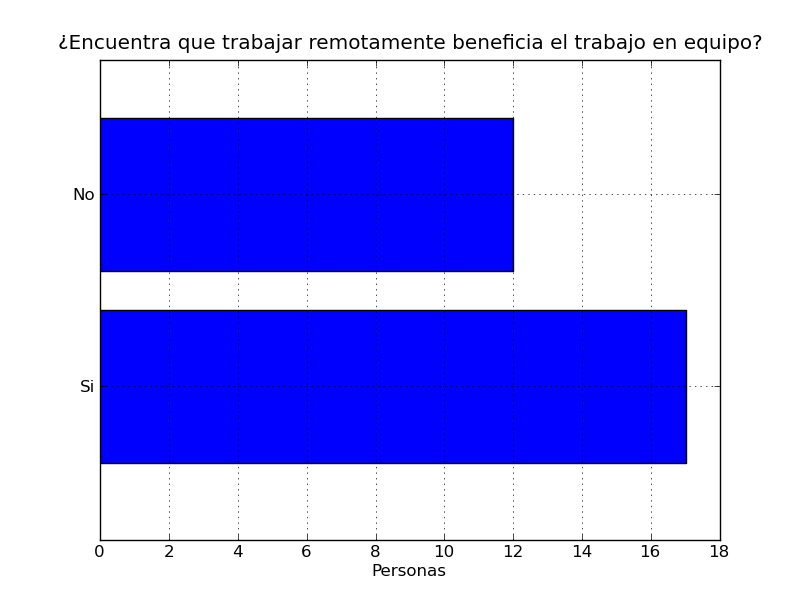
\includegraphics[width=0.8\textwidth]{images/fig4}\\
	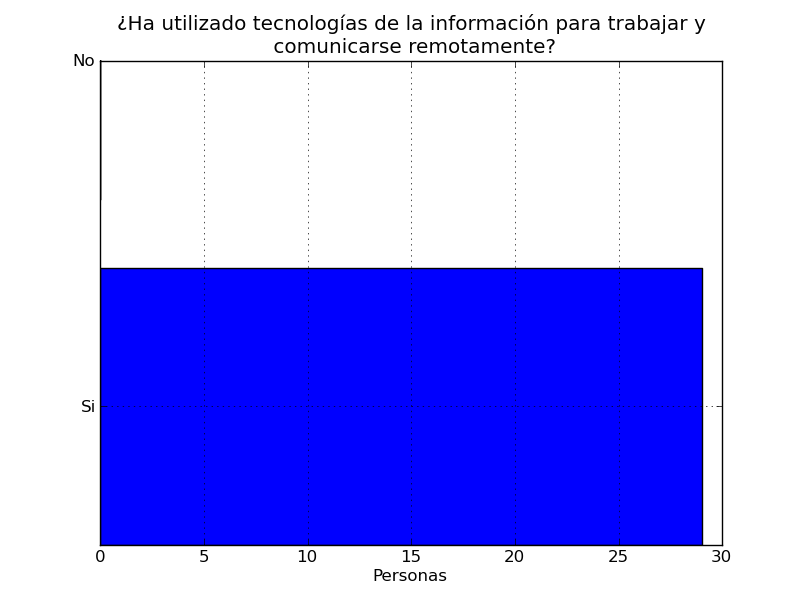
\includegraphics[width=0.8\textwidth]{images/fig5}\\
	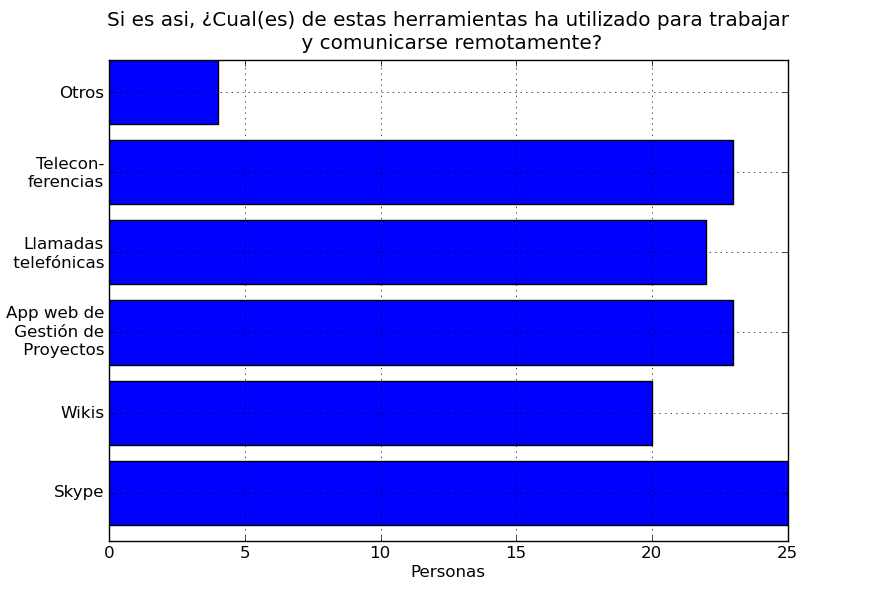
\includegraphics[width=0.8\textwidth]{images/fig6}\\
	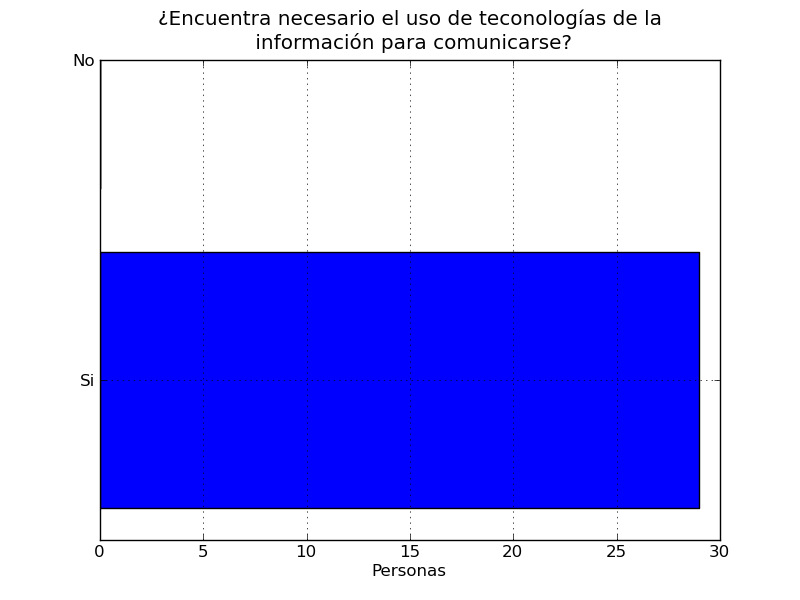
\includegraphics[width=0.8\textwidth]{images/fig7}\\
	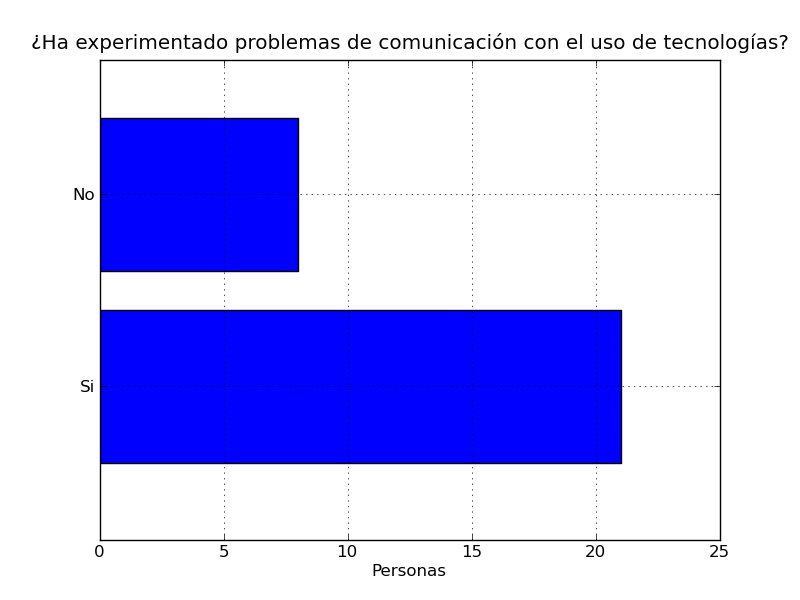
\includegraphics[width=0.8\textwidth]{images/fig8}\\
	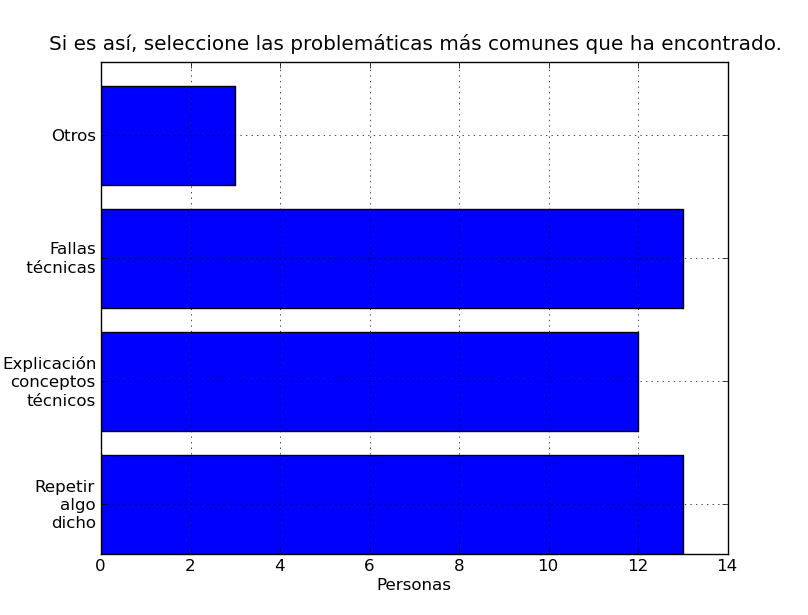
\includegraphics[width=0.8\textwidth]{images/fig9}\\
	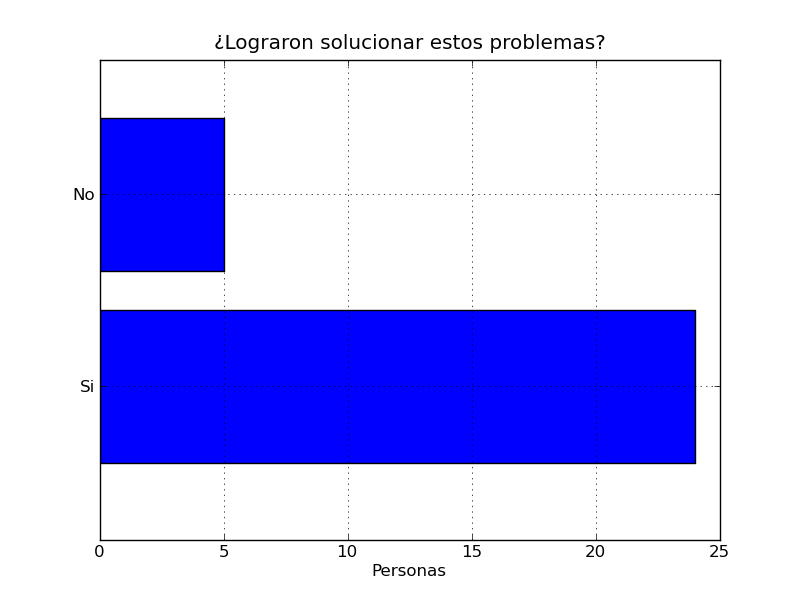
\includegraphics[width=0.8\textwidth]{images/fig10}\\
	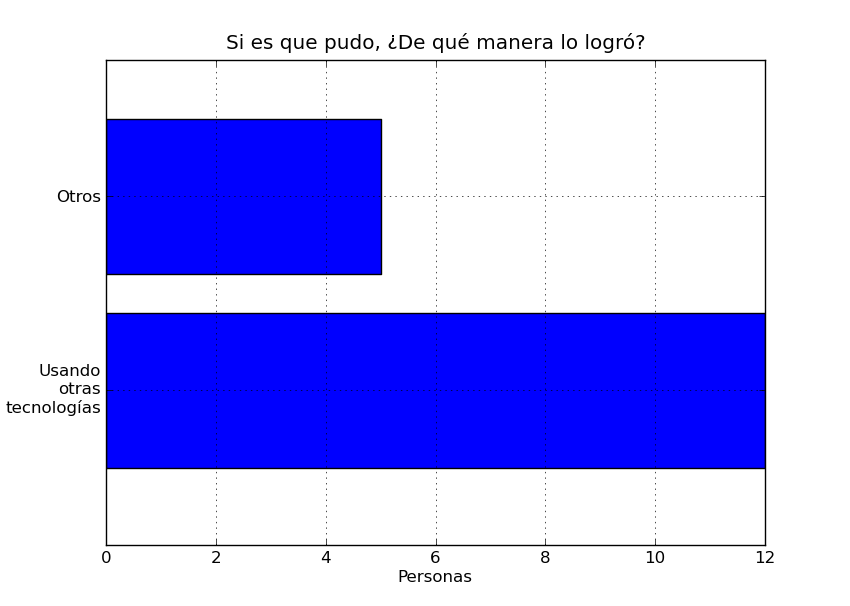
\includegraphics[width=0.8\textwidth]{images/fig11}\\
	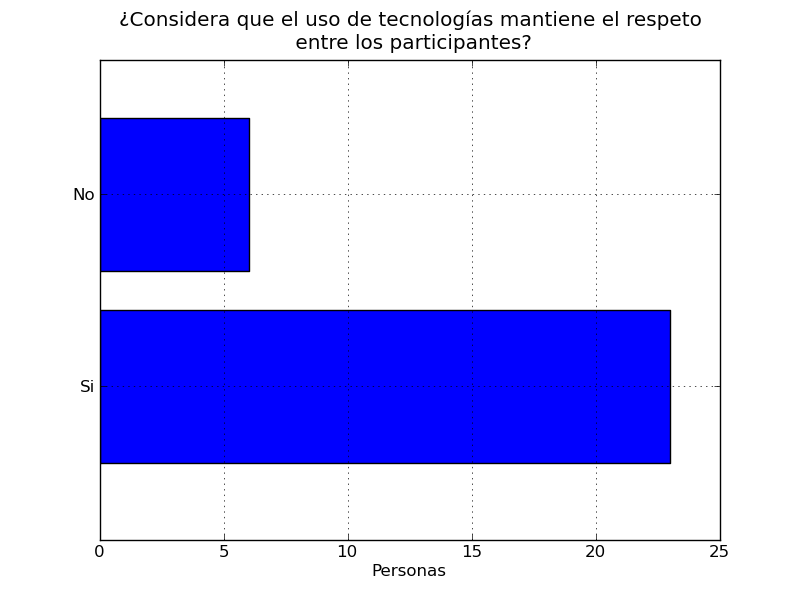
\includegraphics[width=0.8\textwidth]{images/fig12}\\
	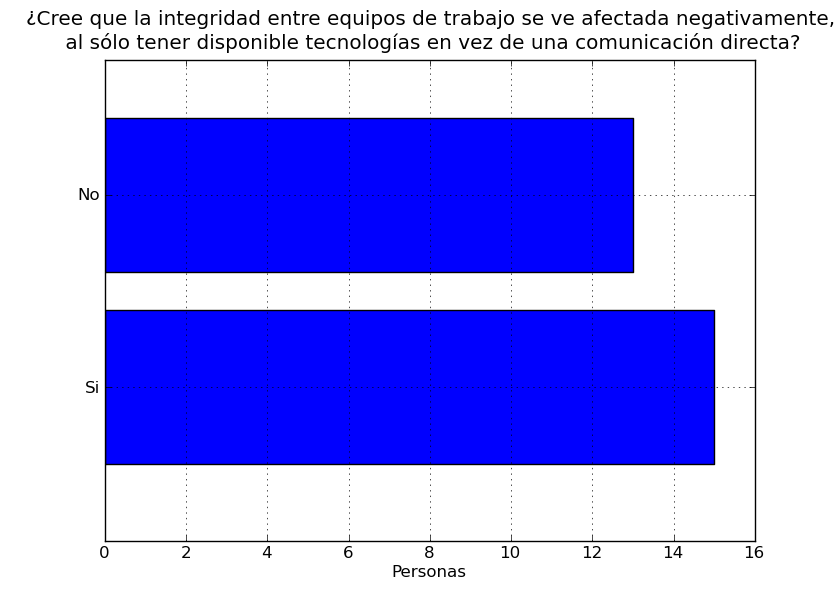
\includegraphics[width=0.8\textwidth]{images/fig13}\\
	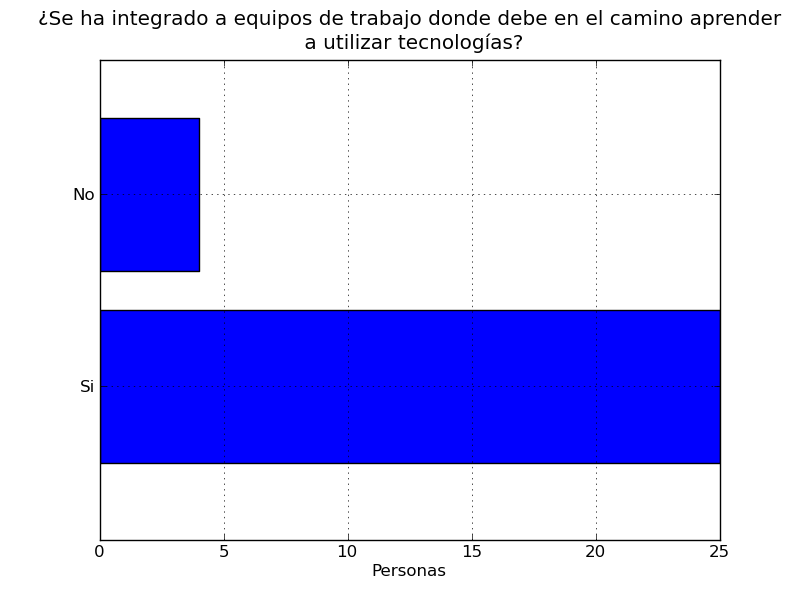
\includegraphics[width=0.8\textwidth]{images/fig14}\\
	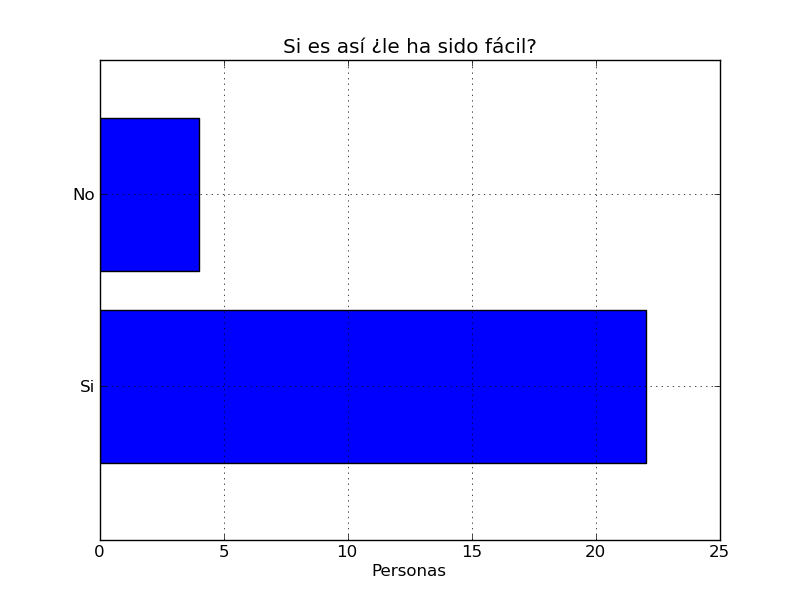
\includegraphics[width=0.8\textwidth]{images/fig15}
\end{center}

El análisis a los presentes resultados es explicado en la siguiente sección.
